\documentclass{article}
\usepackage{graphicx}
\usepackage[style=ieee]{biblatex} % Establecer el estilo de las referencias como IEEE
\usepackage{xcolor}
\usepackage{hyperref}
\usepackage{titletoc}
\usepackage{adjustbox}
\usepackage[spanish]{babel}

\hypersetup{
    colorlinks=true,
    linkcolor=blue, % Color del texto del enlace
    urlcolor=blue % Color del enlace
}

\usepackage{longtable} % Agrega el paquete longtable

\definecolor{mygreen}{RGB}{0,128,0}

\usepackage{array} % Para personalizar la tabla
\usepackage{booktabs} % Para líneas horizontales de mejor calidad
\usepackage{graphicx} % Paquete para incluir imágenes
\usepackage{float}
\usepackage[section]{placeins}

% Definir márgenes
\usepackage[margin=1in]{geometry}

\renewcommand{\contentsname}{\textcolor{mygreen}{Tabla de Contenidos}}

\begin{document}

\begin{titlepage}
    \centering
    % Logo de la Universidad
    
\includegraphics[width=0.48\textwidth]{logo_universidad.png}
    \par\vspace{2cm}

    % Nombre de la Universidad y detalles del curso
    {\Large \textbf{Universidad Nacional de Colombia} \par}
    \vspace{0.5cm}
    {\large Ingeniería de Sistemas y Computación \par}
    {\large 2025966 Lenguajes de Programación (02)\par}
    \vspace{3cm}

    % Detalles del laboratorio y actividad
    {\large \textbf{Tarea 23} \par}
    {\large Compilación y ejecución ejemplos en FLEX.\par}
    \vspace{3cm}

    % Lista de integrantes
    {\large \textbf{Integrantes:} \par}
    \vspace{0.5cm}
    \begin{tabular}{ll}
    Javier Andrés Tarazona Jiménez & jtarazonaj@unal.edu.co \\
    Eder  José Hernández Buelvas   & ehernandezbu@unal.edu.co \\
    Juan Sebastián Muñoz Lemus     & jumunozle@unal.edu.co   \\
    David Felipe Marin Rosas       & dmarinro@unal.edu.co   \\
    \end{tabular}
    \par\vspace{3cm}

    % Fecha
    {\large Mayo 7 de 2025 \par}
\end{titlepage}

\tableofcontents % Inserta la tabla de contenidos

\newpage % Salto de página para separar la tabla de contenidos del contenido del documento

% Contenido del artículo----------------------------------------------------------

%---------------------------------------------------------------------------------
% Intro --------------------------------------------------------------------------
%---------------------------------------------------------------------------------

\section{Introducción}\label{sec:intr}

En el presente trabajo se busca explorar, adaptar y ejecutar programas desarrollados con FLEX, una herramienta ampliamente utilizada para la generación automática de analizadores léxicos, fundamentales en la construcción de compiladores y sistemas de procesamiento de texto. A través de la revisión de ejemplos, su adecuación al entorno de compilación actual, la compilación con herramientas como flex y gcc, y la ejecución con distintos casos de prueba, se pretende comprender el flujo de trabajo que convierte definiciones de patrones léxicos en analizadores funcionales. La experiencia adquirida permitirá relacionar la teoría del análisis léxico —como el uso de expresiones regulares y la definición de tokens— con su aplicación práctica, desarrollando competencias esenciales para enfrentar retos en compilación, transformación de textos y procesamiento automático de lenguajes de programación.
%---------------------------------------------------------------------------------
% Marco Teórico ------------------------------------------------------------------
%---------------------------------------------------------------------------------

\section{Marco Teórico}\label{sec:marc}

\subsection*{Procesador de Lenguaje}

Un procesador de lenguaje es un programa que permite interpretar, traducir o ejecutar instrucciones escritas en lenguajes de programación específicos. Dependiendo de su enfoque, estos procesadores pueden clasificarse principalmente en compiladores, intérpretes o soluciones híbridas, cada uno con particularidades y finalidades concretas.

\subsection*{Compilador}

El compilador es un tipo de procesador de lenguaje que convierte un código fuente escrito en un lenguaje de alto nivel en un programa equivalente en otro lenguaje, comúnmente lenguaje de máquina. Durante este proceso, el compilador identifica y reporta posibles errores presentes en el código original. Además de la fase principal de traducción, se incluyen procesos como:
\begin{itemize}
    \item \textbf{Preprocesador:} Gestiona directivas y macros, preparando el código antes de la compilación.
    \item \textbf{Ensamblador:} Convierte el código intermedio a lenguaje ensamblador o código objeto.
    \item \textbf{Vinculador (Linker):} Une múltiples módulos de código objeto y bibliotecas, generando un ejecutable final.
    \item \textbf{Cargador (Loader):} Se encarga de ubicar el programa en memoria para su ejecución.
\end{itemize}

\subsection*{Intérprete}

Un intérprete, a diferencia del compilador, traduce y ejecuta línea por línea el código fuente directamente en tiempo de ejecución. Aunque suele ser más lento en ejecución que un programa compilado, permite una detección y notificación de errores más detallada.

\subsection*{Procesador Híbrido}

Existen lenguajes que combinan técnicas de compilación e interpretación. Un caso representativo es Java: su código fuente se compila primero a \textit{bytecode}, una forma intermedia, que luego es interpretado y optimizado en tiempo de ejecución mediante compiladores just-in-time (JIT) en la máquina virtual.

\subsection*{Estructura de un Compilador}

La tarea principal de un compilador es transformar el código fuente en un programa destino equivalente en funcionalidad. Este proceso se divide en dos bloques generales: \textbf{análisis} y \textbf{síntesis}.

\begin{itemize}
    \item \textbf{Análisis (Front-End):} Descompone el programa en sus componentes básicos, validando estructura y significado. Genera una forma intermedia del programa y llena una tabla de símbolos con información relevante.
    \item \textbf{Síntesis (Back-End):} Utiliza la representación intermedia y la tabla de símbolos para producir el código de salida en lenguaje de máquina, optimizando su rendimiento.
\end{itemize}

Las fases principales comprenden:
\begin{itemize}
    \item Análisis léxico: Segmenta el flujo de caracteres en unidades mínimas denominadas tokens.
    \item Análisis sintáctico: Estructura los tokens en un árbol o estructura gramatical.
    \item Análisis semántico: Verifica la coherencia lógica del código.
    \item Generación de código intermedio y optimización: Produce y refina una representación que será traducida a lenguaje de máquina.
    \item Generación de código final: Traduce la representación intermedia en instrucciones específicas para el hardware destino.
\end{itemize}

\subsection*{Análisis Léxico}

Esta fase inicial, conocida también como \textit{scanner}, convierte el texto del programa en bloques significativos denominados lexemas. Cada lexema se asocia a un token, compuesto por un nombre simbólico y un valor de atributo. Estos tokens permiten a la siguiente fase del compilador trabajar con unidades sintácticas claras, eliminando elementos irrelevantes como espacios o comentarios.
\subsection*{Flex como Herramienta de Análisis Léxico}

\texttt{Flex} es un generador de analizadores léxicos utilizado para crear programas que identifican patrones textuales dentro de un flujo de entrada. Facilita la construcción de analizadores robustos que forman parte de compiladores u otras herramientas de procesamiento de texto. Flex transforma la especificación de los patrones en código C que clasifica los caracteres de entrada, produciendo tokens que simplifican las fases posteriores del análisis.
\subsection*{Expresiones Regulares}

Un lenguaje se puede definir como un conjunto de cadenas de símbolos de un alfabeto finito. Las expresiones regulares permiten describir lenguajes de forma compacta. Sus principales operaciones son:
\begin{itemize}
    \item \textbf{Símbolo:} Cada símbolo del alfabeto define un lenguaje que contiene solo ese símbolo.
    \item \textbf{Alternación ($|$):} Combina dos expresiones para incluir cadenas de cualquiera de los dos lenguajes.
    \item \textbf{Concatenación:} Une dos expresiones regulares para formar cadenas compuestas.
    \item \textbf{Epsilon ($\epsilon$):} Representa el lenguaje que solo contiene la cadena vacía.
    \item \textbf{Cierre de Kleene ($*$):} Genera todas las combinaciones posibles de cero o más repeticiones de una expresión.
\end{itemize}

Estas herramientas son la base para definir patrones de tokens dentro de un analizador léxico.


\subsection{Contextualización del problema}

En el desarrollo de compiladores, la fase de análisis léxico es vital para segmentar y clasificar correctamente la entrada de código fuente, usar herramientas como Flex permite automatizar esta tarea de forma eficiente y estandarizada. La capacidad de generar analizadores robustos con expresiones regulares facilita la detección y estructuración de tokens, optimizando el proceso de traducción de lenguajes y el flujo de compilación. Este trabajo se centra en comprender, ajustar y ejecutar ejemplos con Flex, reforzando la relación entre teoría y práctica en el procesamiento de lenguajes.



%---------------------------------------------------------------------------------
% Descripción y Justificación del Problema a Resolver ----------------------------
%---------------------------------------------------------------------------------

\section{Descripción y Justificación del Problema a Resolver}\label{sec:descr}

El propósito de esta actividad es profundizar en el uso, compilación y ejecución de programas construidos con \textbf{FLEX}, una herramienta muy empleada en la elaboración de analizadores léxicos dentro del ámbito de los compiladores. FLEX posibilita la definición de patrones basados en expresiones regulares para interpretar y manipular textos, generando de forma automática código en lenguaje C que implementa el analizador léxico de manera eficiente.

El trabajo contempla varias tareas clave:
\begin{itemize}
    \item \textbf{Estudio de ejemplos proporcionados:} Examinar detalladamente los archivos que describen analizadores léxicos mediante reglas y expresiones regulares.
    \item \textbf{Adaptación:} Modificar los ejemplos cuando sea necesario para garantizar su correcta compilación y funcionamiento en el entorno actual.
    \item \textbf{Construcción y prueba:} Emplear herramientas como \texttt{flex} y \texttt{gcc} para generar los analizadores y ejecutar pruebas con distintos insumos.
    \item \textbf{Registro y análisis:} Documentar el comportamiento observado en al menos tres escenarios de prueba distintos, evaluando los resultados obtenidos.
\end{itemize}

\section*{Justificación}

Dominar herramientas como FLEX resulta esencial para quienes estudian Ingeniería de Sistemas o Ciencias de la Computación, dado que los analizadores léxicos constituyen una etapa fundamental en el desarrollo de compiladores y sistemas que procesan lenguajes. Este trabajo contribuye a:
\begin{itemize}
    \item \textbf{Comprender los principios del análisis léxico:} A través de la práctica con expresiones regulares, definición de tokens y su procesamiento automático.
    \item \textbf{Aplicar la teoría a casos reales:} Conectando lo aprendido en clase con ejemplos funcionales.
    \item \textbf{Manejar herramientas estándares:} Adquiriendo experiencia práctica con utilidades ampliamente utilizadas en la industria del software.
    \item \textbf{Resolver inconvenientes de compatibilidad:} Enfrentando situaciones reales de ajuste de código y entorno.
\end{itemize}

Asimismo, las habilidades desarrolladas mediante esta práctica resultan aplicables en otras áreas, como la construcción de sistemas que interpretan o transforman información textual, fortaleciendo competencias prácticas y transferibles a diversos proyectos de computación.

\subsection{Objetivo Principal}

Comprender y aplicar el uso de FLEX para crear, compilar y ejecutar analizadores léxicos, relacionando teoría y práctica en el contexto del desarrollo de compiladores y procesamiento de texto.

%---------------------------------------------------------------------------------
% Diseño de la solución ---------------------------------------------------------
%---------------------------------------------------------------------------------

\section{Diseño de la solución}\label{sec:dis}

La aplicación propuesta tiene como fin ofrecer un entorno interactivo para explorar, modificar y ejecutar programas desarrollados con \texttt{FLEX}. Está orientada tanto a estudiantes como a usuarios interesados en experimentar con la creación de analizadores léxicos, facilitando la comprensión de su funcionamiento y la validación de resultados en distintos contextos de entrada.

\subsection*{Características Principales}

Las funciones clave que conforman la herramienta son:

\begin{enumerate}
    \item \textbf{Gestor de Ejemplos:} Permite importar programas escritos en \texttt{FLEX} desde archivos locales o repositorios, y realizar modificaciones mediante una interfaz de edición integrada.
    \item \textbf{Compilación Automatizada:} Emplea \texttt{flex} para generar el código en C y \texttt{gcc} para compilarlo, gestionando los mensajes de error y proporcionando retroalimentación clara.
    \item \textbf{Módulo de Pruebas:} Ofrece la opción de definir múltiples entradas de prueba, ejecutarlas y recolectar las salidas del analizador léxico generado.
    \item \textbf{Panel de Resultados:} Visualiza de manera organizada los resultados de cada ejecución, facilitando la comparación entre diferentes escenarios.
    \item \textbf{Registro de Cambios:} Guarda un historial de modificaciones aplicadas a los programas y documenta el efecto que estos cambios tienen sobre los resultados de ejecución.
\end{enumerate}

\subsection*{Arquitectura General}

La estructura de la aplicación se divide en módulos interconectados:

\begin{itemize}
    \item \textbf{Módulo de Importación y Edición:} Facilita la selección, carga y edición de archivos FLEX.
    \item \textbf{Módulo de Construcción:} Coordina la generación de código y la compilación, manejando incidencias que puedan surgir durante el proceso.
    \item \textbf{Módulo de Ejecución:} Ejecuta los programas compilados con diferentes entradas de prueba definidas por el usuario.
    \item \textbf{Módulo de Resultados:} Presenta las salidas de forma comprensible y comparativa.
    \item \textbf{Módulo de Bitácora:} Documenta ajustes y observaciones para futuras consultas.
\end{itemize}

\subsection*{Flujo de Operación}

El proceso de uso se desarrolla de la siguiente forma:
\begin{enumerate}
    \item El usuario selecciona y abre un programa de ejemplo.
    \item Modifica el código si es necesario mediante la interfaz de edición.
    \item Lanza la compilación con \texttt{flex} y \texttt{gcc} desde el módulo de construcción.
    \item Define casos de entrada para poner a prueba el analizador léxico.
    \item Ejecuta las pruebas y revisa los resultados generados.
    \item Registra comentarios y ajustes aplicados para análisis posteriores.
\end{enumerate}


\subsection{Metodología}

La metodología de trabajo propuesta combina actividades prácticas con análisis reflexivo para garantizar un aprendizaje integral. Se seguirá la siguiente secuencia:

\begin{itemize}
    \item \textbf{Exploración Inicial:} Selección y revisión de programas FLEX disponibles, comprendiendo la estructura y la lógica de cada ejemplo.
    \item \textbf{Adaptación:} Realización de ajustes sobre los ejemplos para que sean compatibles con el entorno de compilación actual.
    \item \textbf{Construcción del Analizador:} Generación automática del código C a partir del archivo FLEX y compilación del ejecutable usando \texttt{gcc}.
    \item \textbf{Definición de Escenarios:} Elaboración de al menos tres casos de prueba para verificar el comportamiento del analizador léxico en distintas situaciones.
    \item \textbf{Ejecución y Verificación:} Pruebas controladas para observar cómo responde el programa ante cada entrada definida.
    \item \textbf{Análisis y Registro:} Revisión de los resultados, documentación de los ajustes realizados y de las conclusiones obtenidas en cada iteración.
\end{itemize}

%---------------------------------------------------------------------------------
% Código Fuente ---------------------------------------------------------
%---------------------------------------------------------------------------------

\section{Código Fuente}\label{sec:cod}

El código fuente se encuentra en la carpeta ProgramasEnFLEX ubicada en la Biblioteca digital del curso.

%---------------------------------------------------------------------------------
% Manual Usuario ---------------------------------------------------------
%---------------------------------------------------------------------------------

\section{Manual Usuario}\label{sec:man_u}

\section*{Manual de Usuario}

Este manual tiene como propósito orientar al usuario durante el proceso de descarga, instalación, configuración y ejecución de ejemplos desarrollados con \texttt{FLEX}, una herramienta utilizada para la generación de analizadores léxicos. A continuación se detallan los pasos de forma clara y práctica.

\subsection*{1. Descarga e Instalación de FLEX}

\begin{enumerate}
    \item Acceda al siguiente enlace: \url{http://gnuwin32.sourceforge.net/packages/flex.htm}
    \item Descargue el instalador disponible.
    \item Abra el archivo descargado y siga las instrucciones del asistente:
    \begin{enumerate}
        \item Haga clic en ``Siguiente''.
        \item Lea y acepte los términos de la licencia.
        \item Escoja la ubicación de instalación y presione ``Siguiente''.
        \item Elija el tipo de instalación y los componentes deseados.
        \item Configure la creación de accesos directos en el menú de inicio.
        \item Confirme la instalación y haga clic en ``Instalar''.
        \item Finalice el proceso seleccionando ``Terminar''.
    \end{enumerate}
\end{enumerate}

\subsection*{2. Instalación de MinGW}

\begin{enumerate}
    \item Visite: \url{https://sourceforge.net/projects/mingw/files/}
    \item Descargue el archivo ``mingw-get-setup''.
    \item Ejecute el instalador y siga estos pasos:
    \begin{enumerate}
        \item Seleccione ``Instalar''.
        \item Avance presionando ``Continuar'' cuando se le solicite.
        \item Marque los paquetes \texttt{mingw32-base} y \texttt{mingw32-gcc-g++}.
        \item Presione ``Instalar'' y luego ``Aplicar cambios''.
    \end{enumerate}
\end{enumerate}

\subsection*{3. Instalación de Bison}

\begin{enumerate}
    \item Ingrese a: \url{http://gnuwin32.sourceforge.net/packages/bison.htm}
    \item Descargue el archivo ``bison-2.4-setup''.
    \item Ejecute el instalador y avance siguiendo estos pasos:
    \begin{enumerate}
        \item Lea y acepte los términos de uso.
        \item Marque los componentes ``Binarios'', ``Documentación'' y ``Archivos de desarrollo''.
        \item Escoja la carpeta de destino.
        \item Configure la creación de accesos directos.
        \item Haga clic en ``Instalar'' y finalice con ``Terminar''.
    \end{enumerate}
\end{enumerate}

\subsection*{4. Configuración de Variables de Entorno (PATH)}

\begin{enumerate}
    \item Abra el Panel de Control y acceda a ``Sistema''.
    \item Seleccione ``Configuración avanzada del sistema''.
    \item Haga clic en ``Variables de entorno''.
    \item Localice la variable ``Path'' y presione ``Editar''.
    \item Seleccione ``Nuevo'' y agregue la ruta a la carpeta \texttt{bin} de MinGW (por ejemplo, \texttt{C:\textbackslash MinGW\textbackslash bin}).
    \item Si dispone de otras carpetas relevantes (por ejemplo, \texttt{MinGW32}), añádalas también.
    \item Confirme los cambios y reinicie el equipo para aplicar la nueva configuración.
\end{enumerate}

\subsection*{5. Copia de Librerías Necesarias}

\begin{enumerate}
    \item Navegue a la carpeta de instalación de GnuWin32 y ubique la librería requerida por MinGW.
    \item Copie la librería.
    \item Péguela en la carpeta de \texttt{MinGW} correspondiente para asegurar la correcta vinculación durante la compilación.
\end{enumerate}

\subsection*{6. Ejecución de un Programa FLEX}

\begin{enumerate}
    \item Abra una terminal (símbolo del sistema o terminal de preferencia).
    \item Navegue a la carpeta donde se encuentra el archivo FLEX a compilar.
    \item Ejecute el siguiente comando para generar el código fuente C:
    \begin{verbatim}
flex <nombre_del_archivo>.l
    \end{verbatim}
    Por ejemplo:
    \begin{verbatim}
flex 01_01_simple.l
    \end{verbatim}

    \item Compile el archivo generado con:
    \begin{verbatim}
gcc lex.yy.c -lfl
    \end{verbatim}

    Esto producirá un archivo ejecutable (\texttt{a.exe}) y el archivo intermedio \texttt{lex.yy.c}.

    \item Finalmente, ejecute el programa con:
    \begin{verbatim}
.\a.exe
    \end{verbatim}

    Si todo se realizó correctamente, el analizador léxico procesará la entrada según el programa definido.
\end{enumerate}


%---------------------------------------------------------------------------------
% Manual Técnico ---------------------------------------------------------
%---------------------------------------------------------------------------------

%---------------------------------------------------------------------------------
% Experimentación ---------------------------------------------------------
%---------------------------------------------------------------------------------

\section{Experimentación}\label{sec:exp}

Para desarrollar este trabajo se siguió una secuencia estructurada de pasos que permitió validar el funcionamiento de los programas escritos en \texttt{FLEX}. El proceso se dividió en las siguientes etapas:

\begin{itemize}
    \item \textbf{Revisión de materiales:} Se exploraron los programas de ejemplo, identificando su propósito y estructura.
    \item \textbf{Compilación preliminar:} Cada archivo fue procesado con \texttt{flex} para generar el código fuente en C, y luego compilado con \texttt{gcc} para producir un ejecutable funcional. Se documentaron cambios o correcciones requeridas.
    \item \textbf{Pruebas en diversos casos:} Cada programa se evaluó bajo al menos tres condiciones de entrada distintas, incluyendo datos simples, símbolos especiales y casos más complejos.
    \item \textbf{Registro de observaciones:} Se anotaron los resultados obtenidos, identificando cualquier desviación y proponiendo ajustes en caso de ser necesarios.
    \item \textbf{Síntesis de hallazgos:} Finalmente, se reunieron conclusiones generales sobre la experiencia de uso de \texttt{FLEX} y sus posibles limitaciones.
\end{itemize}

\subsection{Análisis de resultados del ejemplo \texttt{01\_01\_simple.l}}

\subsubsection{Escenario 1: }

Este primer programa actúa como un eco: lee cualquier carácter introducido por el usuario y lo muestra en pantalla sin aplicar transformaciones. La expresión regular utilizada (\verb|.| o \verb|\n|) garantiza que todo carácter, incluidos saltos de línea, sea capturado.

\textbf{Entrada:}  
\begin{verbatim}
Hola mundo
FLEX es genial
\end{verbatim}

\begin{figure}[H]
    \centering
    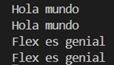
\includegraphics[width=0.5\linewidth]{image.png}
\end{figure}

\textbf{Observación:}  
La salida reflejó fielmente la entrada. Cada línea se imprimió tal como se introdujo, demostrando que el analizador funciona correctamente para casos básicos sin símbolos especiales.

\subsubsection{Escenario 2: }

\textbf{Entrada:}  
\begin{verbatim}
¡Hola, cómo estás?
Esto es FLEX.
\end{verbatim}

\begin{figure}[H]
    \centering
    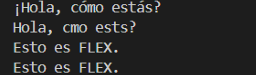
\includegraphics[width=0.5\linewidth]{image2.png}
\end{figure}

\textbf{Observación:}  
Se detectaron inconvenientes con algunos caracteres acentuados. Signos como ``¡'' fueron reconocidos y letras con tilde se mostraron incorrectamente o no aparecieron. Esto sugiere que el programa está limitado a un alfabeto ASCII y requiere ajustes para admitir entradas codificadas en UTF-8.

\subsubsection{Escenario 3: }

\textbf{Entrada:}  
\begin{verbatim}
Línea uno

Línea tres
\end{verbatim}
\begin{figure}[H]
    \centering
    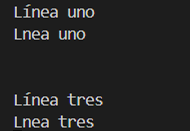
\includegraphics[width=0.5\linewidth]{image3.png}
\end{figure}
\textbf{Observación:}  
En este caso, el programa replicó algunas líneas y omitió caracteres con tilde. El comportamiento muestra que se deben revisar detalles de la configuración de entrada/salida y codificación para evitar duplicados y pérdidas de información.

\subsection{Análisis de resultados del ejemplo \texttt{01\_03\_frases.l}}

Este segundo programa añade lógica para identificar categorías gramaticales en frases simples, como verbos, pronombres, adverbios y conjunciones. Las palabras que no encajan en las reglas predefinidas se consideran sustantivos potenciales.

\subsubsection{Escenario 1: }

\textbf{Entrada:}  
\begin{verbatim}
I am very calm.
She has a book.
\end{verbatim}

\begin{figure}[H]
    \centering
    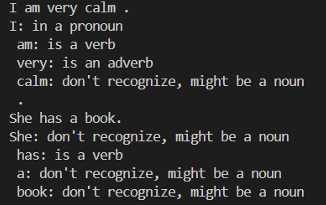
\includegraphics[width=0.5\linewidth]{image4.png}
\end{figure}

\textbf{Observación:}  
El analizador clasificó correctamente los pronombres y verbos, e identificó ``very'' como adverbio. Sin embargo, palabras como ``calm'' y ``book'' no coincidieron con ninguna regla y se marcaron como sustantivos genéricos. El programa logra una categorización básica, pero podría ampliarse para manejar un vocabulario mayor.

\subsubsection{Escenario 2: }

\textbf{Entrada:}  
\begin{verbatim}
The sky is blue.
My dog runs quickly.
\end{verbatim}
\begin{figure}[H]
    \centering
    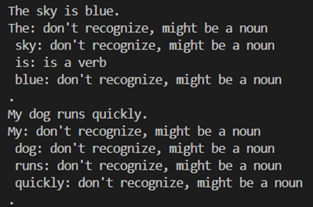
\includegraphics[width=0.5\linewidth]{image5.png}
\end{figure}

\textbf{Observación:}  
En este caso, palabras como ``is'' y ``runs'' fueron reconocidas como verbos, y ``quickly'' como adverbio. Sin embargo, ``The'' y ``sky'' quedaron como palabras no clasificadas. Esto muestra la necesidad de expandir las expresiones regulares para cubrir artículos, preposiciones o sustantivos frecuentes.

\subsubsection{Escenario 3: }


\textbf{Entrada:}  
\begin{verbatim}
¿Dónde está mi perro?
Él corre detrás de mí.
\end{verbatim}

\begin{figure}[H]
    \centering
    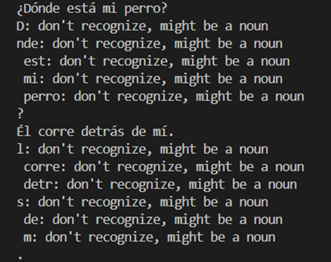
\includegraphics[width=0.5\linewidth]{image6.png}
\end{figure}

\textbf{Observación:}  
El analizador presentó limitaciones para procesar tildes y signos como ``¿''. Palabras clave como ``detrás'', ``mi'' o ``mí'' no fueron identificadas según su categoría correcta (preposición o pronombre). Es evidente que el soporte de caracteres extendidos y la ampliación de reglas gramaticales son mejoras necesarias.

\subsubsection{Conclusiones}

El proceso experimental permitió comprobar que \texttt{FLEX} es una herramienta efectiva para generar analizadores léxicos funcionales en casos sencillos y bien definidos. Sin embargo, se identificaron restricciones importantes al manejar caracteres especiales y palabras con tildes, debido a configuraciones de codificación limitadas o reglas incompletas.

Se recomienda realizar ajustes en las expresiones regulares y utilizar codificaciones que permitan trabajar con Unicode o UTF-8 para mejorar la compatibilidad. Además, ampliar el conjunto de patrones gramaticales optimizaría la clasificación de palabras en textos más complejos.

En general, la práctica mostró la versatilidad de \texttt{FLEX} para tareas de procesamiento de texto, destacando su potencial en entornos educativos y de investigación, siempre que se complemente con reglas y configuraciones acordes a las necesidades del lenguaje que se desea analizar.

\section{Referencias}
\renewcommand{\refname}{}

\begin{thebibliography}{9}
\bibitem{1}
Aho, A. V., Lam, M. S., Sethi, R., \& Ullman, J. D. (2007). \textit{Compilers: Principles, Techniques, and Tools} (2nd ed.). Pearson Education.
\bibitem{2}
Appel, A. W., \& Palsberg, J. (2004). \textit{Modern Compiler Implementation in Java} (2nd ed.). Cambridge University Press.
\bibitem{3}
Westes, B. (n.d.). \textit{flex: The fast lexical analyzer}. GitHub. Retrieved December 13, 2024, from \url{https://github.com/westes/flex}

\end{thebibliography}

\end{document}